 \documentclass[english]{article}

\usepackage{babel}
\usepackage{graphicx}
\usepackage{times}
\usepackage{pifont}
\usepackage[margin=1in]{geometry}
\usepackage{eurosym}
\usepackage{fancyhdr}
\usepackage[hidelinks]{hyperref}
\usepackage{float}

\pagestyle{fancy}
\fancyhf{}


%HEADER
%**************************************************************************************
\pagestyle{fancy}
\fancyhf{}
%**************************************************************************************
\lhead{Microsensors and mechanics}		 	 
\rhead{MEMS pressure sensor} 
\lfoot{EFA12SF}
\cfoot{\thepage}
\rfoot{Alexey Tukalo}
%**************************************************************************************

\date{}
\setlength\parindent{0pt}

\begin{document}

\begin{titlepage}

\begin{flushleft}
Seminar work report\\
Course: Microsensors and mechanics 2015\\
Class: EFA12SF, \\
Student: Alexey Tukalo,\\
Date: 07.11.2015
\end{flushleft}

\vspace{6.5cm}
	\centering
	{\scshape\LARGE MEMS pressure sensor \par}
	\small for Microsensors and mechanics\\
	\vspace{0.5cm}
	
\includegraphics{savonia.jpg}
\end{titlepage}

\tableofcontents
\setcounter{page}{0}
\newpage


\setcounter{tocdepth}{2}




%MAIN CONTENT ******************************************************************************************************************

\section{Introduction}

Pressure is a physical quantity which describes an amount of force applied to every single part of the area in a direction perpendicular to the surface. The formula \ref{eq:pressure} is mathematical representation of the definition. \cite{types}\\

\begin{equation} 
P = \frac{F}{A}\label{eq:pressure}
\end{equation}\\

Pressure sensors are one of the most popular and developed sensor type, it become spread especially wide in its MEMS realisation. We are literally surrounded by various number of pressure sensor in every day devises and huge industrial solutions. There are several different technologies which allows to build pressure sensors, all of them has their own strong and weak sides. \\

Microelectromechanical Systems is complex of mechanical components and devices in size from a few micrometers to a few hundreds of microns. Many different types of sensors have MEMS realisations for example: pressure sensors, accelerometers, gyroscopes and gyrometers. It is also possible to produce actuators in MEMS format. Typical MEMS actuators are microengines, microlocks and discriminators.\cite{mems}\\

\section{General principle and main types of the pressure sensor}
There are three main types of pressure sensors:

\begin{enumerate}
\item Gauge pressure sensor - measures a value relatively to atmospheric pressure.
\item Absolute pressure sensor - use absolute vacuum as origin.
\item Differential pressure sensor - compare pressure with some variable value, can be used to measure difference between two pressure.
\end{enumerate}

\subsection{Sensor types}

\subsubsection{The gauge pressure sensor}

This type of sensors contains the ventilation hole on the back-side which connects the sensitive part with the atmosphere and the pressure applied to the front-side of the devise is measured with reference to it, Pic. \ref{fig:gauge}.\\

\begin{figure}[H]
\centerline{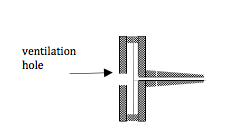
\includegraphics[scale=1]{PressureSensors/gauge}}
\caption{The gauge type pressure sensor \label{fig:gauge}}
\end{figure}

This kind of sensors should not be used for vessels with aggressive liquids and hazardous gases, because only sensor would separate such dangerous substances from  "outside world" and damage of the sensor is able to provoke an accident. This type of sensors also is not suitable for the high pressure tanks.\cite{spd} \\

The image \ref{fig:gaugePhoto} demonstrates an example of gauge sensor.

\begin{figure}[H]
\centerline{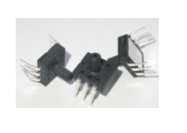
\includegraphics[scale=0.7]{PressureSensors/gaugePhoto}}
\caption{The gauge type pressure sensor example \label{fig:gaugePhoto}}
\end{figure}

\subsubsection{The absolute pressure sensor}

This kind of sensors has reference chamber with pressure close to vacuum inside. Of course it is impossible to create a chamber with an absolute vacuum, it usually has 25.10-3 Torr or 5.10-4 PSI for Smartec sensors, Pic \ref{fig:abs}.\\

\begin{figure}[H]
\centerline{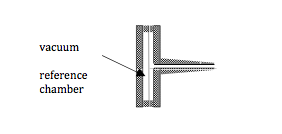
\includegraphics[scale=1]{PressureSensors/abs}}
\caption{The absolute type pressure sensor \label{fig:abs}}
\end{figure}

A very important thing is that the vacuum must be very high to avoid an influence of the temperatures difference, anyway this kind of sensors has temperature limits and can be inaccurate outside the range.\\

The absolute pressure sensor much more safe than gauge one, but it is more expensive because of vacuum chamber.\cite{spd}\\

The image \ref{fig:absPhoto} shows an example of absolute sensor.

\begin{figure}[H]
\centerline{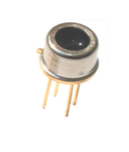
\includegraphics[scale=0.7]{PressureSensors/absPhoto}}
\caption{The absolut type pressure sensor example \label{fig:absPhoto}}
\end{figure}

\subsubsection{The differential pressure sensor}
The differential pressure sensor has two inputs, one of them is called negative and another one positive. This type of sensors is able to measure difference of the pressure between the ports, Pic \ref{fig:diff}.\cite{spd}

\begin{figure}[H]
\centerline{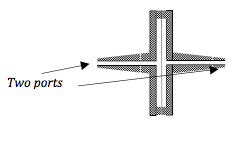
\includegraphics[scale=1]{PressureSensors/diff}}
\caption{The differential type of pressure sensor \label{fig:diff}}
\end{figure}

The image \ref{fig:diffPhoto} shows an example of absolute sensor.

\begin{figure}[H]
\centerline{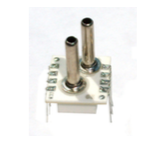
\includegraphics[scale=0.7]{PressureSensors/diffPhoto}}
\caption{The differential type pressure sensor example \label{fig:diffPhoto}}
\end{figure}


\subsection{General principles}

It is also possible to use physical principle of the sensors for classification. The table \ref{tab:types} contains the most complete information about weak and strong sides of different solutions.\\

In general the sensors are based on changes of electromagnetic or other properties of material due to applied force. For example resistive pressure sensors are based on metals with an impedance sensible for stress. The resistance of the material is dependent from an amount of force applied to it.\cite{types}\\

Another approach is to use materials with an ability to emit energy as response to applied force. Piezoelectric pressure sensors are perfect example of the idea. The sensors are based on the Silicon on Insulator (SOI). Force applied to this kind of crystals provoke polarisation and generation of charge proportional to the stress. Piezoelectric effect is typical for quartz, tourmaline, and several other naturally crystals.\cite{piez}\\

Optical and Ultrasonic pressure sensors can be useful to avoid an influence of strong electromagnetic fields. An Optical ones are constructed in the way that pressure applied to them changes an amount of absorbed light in an according with certain transfer function. \cite{optics} Ultrasonic sensors are able to measure pressure via changes of sound speed of sound, the wave length and an attenuation of the waves inside the material on stress.\cite{ultrasonic}

\begin{table}
 \begin{center}
  \caption{Characterisation of different technologies\cite{types}\label{tab:types}}
    \begin{tabular}{ l l l }    
    	\hline
  	   Type  				     & 			Advantages 				& 			Disadvantages  \\ \hline\\
  	   Resistive 				
  	   
  	    & 
  	   
\begin{minipage}{2.5in}									
    \begin{enumerate}
   \item Sensitive
   \item Low cost
   \end{enumerate}
 \end{minipage}  
 
 &
 
\begin{minipage}{2.5in}									
    \begin{enumerate}
   \item High power consumption
   \item Generally detect single contact point
   \item Lack of contact force measurement
   \end{enumerate}
 \end{minipage} 
 
 \\\\\hline
 
 
  	   Piezoresistive 	
  	   
  	   &
  	   
 \begin{minipage}{2.5in}									
    \begin{enumerate}
   \item Low cost
   \item Good sensitivity
   \item Low noise
   \item Simple electronics
   \end{enumerate}
 \end{minipage} 
 
  &
 
\begin{minipage}{2.5in}									
    \begin{enumerate}
   \item Stiff and frail
   \item Nonlinear response
   \item Hysteresis
   \item Temperature sensitive
   \end{enumerate}
 \end{minipage}
 
  \\\\\hline
 
	   Tunnel effect 	
	   
	   &
	   
\begin{minipage}{2.5in}									
    \begin{enumerate}
   \item Sensitive
   \item Physically flexible
   \end{enumerate}
 \end{minipage}  
 
 &
 
\begin{minipage}{2.5in}									
    \begin{enumerate}
   \item Nonlinear response
   \end{enumerate}
 \end{minipage} 
 
 \\\\\hline
 
 	   Capacitive	
 	   
 	   &
 	   
 \begin{minipage}{2.5in}									
    \begin{enumerate}
   \item Sensitive
   \item Low cost
   \item Availability of commercial A/D chips
   \end{enumerate}
 \end{minipage}  
 
 &

\begin{minipage}{2.5in}									
    \begin{enumerate}
   \item Hysteresis
   \item Complex electronics
   \end{enumerate}
 \end{minipage} 
 
 \\\\\hline

 	   Optical			
 	   
 	   &
 	   		
 \begin{minipage}{2.5in}									
    \begin{enumerate}
   \item Sensitive
   \item Physically flexible
   \item Fast
   \item No interconnections
   \end{enumerate}
 \end{minipage} 
 
  &

\begin{minipage}{2.5in}									
    \begin{enumerate}
   \item Loss of light by micro bending chirping
   \item Power consumption
   \item Complex computations
   \end{enumerate}
 \end{minipage} 
 
 \\\\\hline
 
 	   Ultrasonic		
 	   
 	   &
 	   
 	   		 \begin{minipage}{2.5in}									
    \begin{enumerate}
   \item Fast dynamic response
   \item Good force resolution
   \end{enumerate}
 \end{minipage}  
 
 &
 
\begin{minipage}{2.5in}									
    \begin{enumerate}
   \item Limited utility at low frequency
   \item Complex electronics
   \item Temperature sensitive
   \end{enumerate}
 \end{minipage} 
 
 \\\\\hline
 
 	   Magnetic	
 	   	
 	   &
 	   
 	   		 \begin{minipage}{2.5in}									
    \begin{enumerate}
   \item High sensitivity
   \item Good dynamic range
   \item No mechanical hysteresis
   \item Physical robustness
   \end{enumerate}
 \end{minipage}  
 
 &
 
\begin{minipage}{2.5in}									
    \begin{enumerate}
   \item Suffer from magnetic interference
   \item Complex computations
   \item Somewhat bulky
   \item Power consumption
   \end{enumerate}
 \end{minipage} 
 
 \\\\\hline
 
 	   Piezoelectric		
 	   
 	   &
 	   
 	   	 \begin{minipage}{2.5in}									
    \begin{enumerate}
   \item Dynamic response
   \item High bandwidth
   \end{enumerate}
 \end{minipage}  
 
 &
 
\begin{minipage}{2.5in}									
    \begin{enumerate}
   \item Temperature sensitive
   \item Not so robust electrical connection
   \end{enumerate}
 \end{minipage} 
 
 \\\\\hline
 
 	   Conductive rubber 
 	   
 	   &
 	   
 	   \begin{minipage}{2.5in}									
    \begin{enumerate}
   \item Physically flexible
   \end{enumerate}
 \end{minipage} 
 
  &
  
\begin{minipage}{2.5in}									
    \begin{enumerate}
   \item Mechanical hysteresis
   \item Nonlinear response
   \end{enumerate}
 \end{minipage} 
 
 \\\\\hline
    \end{tabular}
 \end{center}
\end{table}

\section{Main applications of the pressure sensor}

Pressure sensors have a wide area of application in different fields. Usually, they are used to monitor pressure, flow or level of gases and liquids inside tubes or tanks, the sensors are also able to detect physical contact, the touch's position and power. \cite{inf}

\subsection{Touch detection}

Pressure sensors can be used for accurate identification of position and amount of applied force to the spot. The technology can be used in mobile devices \cite{touch}. Unfortunately, pressure sensors are not able to detect multiple touches precisely, that's why usually they are used for accurate detection of the force applied to the spot, but exact position of the point is measured by other technology, this kind of approach is used by Apple 3D Touch \cite{apple} and graphical tablets Pic. \ref{fig:wacom}. \cite{wacom} In case of graphical tablet they use network of electromagnetic receivers to calculate an exact position of the electromagnetic transducer inside stylus, build into the stylus pressure sensors is used to detect amount of applied force and exact time of the touch, it gives painter an opportunity to  precisely control thickness and shape of lines.

\begin{figure}
\centerline{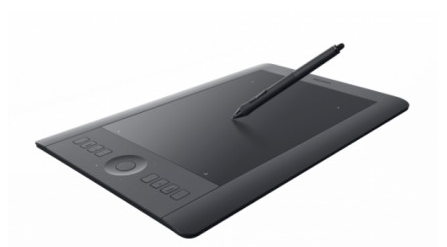
\includegraphics[scale=0.5]{PressureSensors/wacom}}
\caption{Graphical tablet Wacom Intuos Pro Medium\label{fig:wacom} \cite{wacom}}
\end{figure}

\subsection{Automotive Industry}

\begin{figure}
\centerline{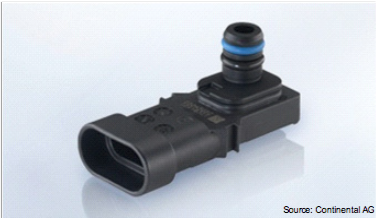
\includegraphics[scale=0.5]{PressureSensors/ems}}
\caption{Picture of a MAP module with an Infineon KP21x sensor inside\label{fig:ems} \cite{inf}}
\end{figure}

Pressure sensors have a lot of application in modern vehicles:

\begin{enumerate}
\item Monitoring of fuel's and oil's amount in tanks
\item Engine management system contains at least one pressure sensor, the sensor is located a manifold and measures the flow of air inside. The data is used to calculate a right amount of fuel for an injection, Pic \ref{fig:ems}.
\item Pressure sensors are used in brake booster, they are very important part of anti-lock breaking system(Pic. \ref{fig:break}), ABS prevents locking of tiers in case of an active breaking.
\item Air bugs are triggered in according with pressure sensor, which is used to detect collision.
\item Diagnostics of particle filters for diesel engines
\end{enumerate}  

Pressure sensors have many other application on automotive industry, which makes car more safe, cheaper, efficient and so on.\cite{inf}

\begin{figure}
\centerline{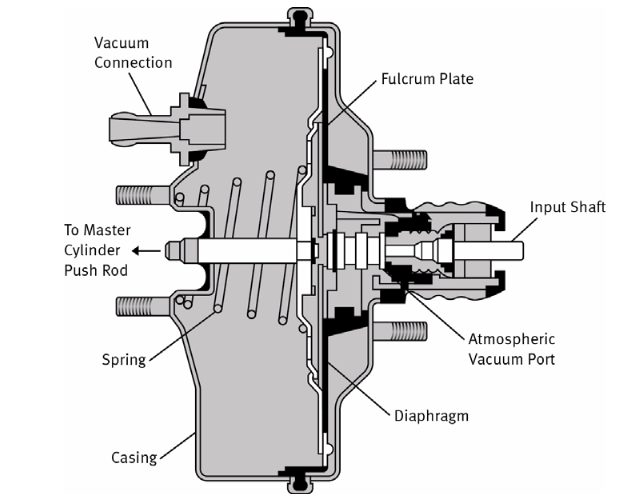
\includegraphics[scale=0.5]{PressureSensors/break}}
\caption{Blueprint of a vacuum power brake booster\label{fig:break} \cite{inf}}
\end{figure}

\subsection{Bio Medical Instrumentation}

Air or liquid flow sensors are especially useful for medical application, they are used in digital blood pressure monitors, lungmotors. Pressure sensors are also used in sphygmomanometer (Pic. \ref{fig:ton}) and various number of other medical devices. \cite{app}

\begin{figure}
\centerline{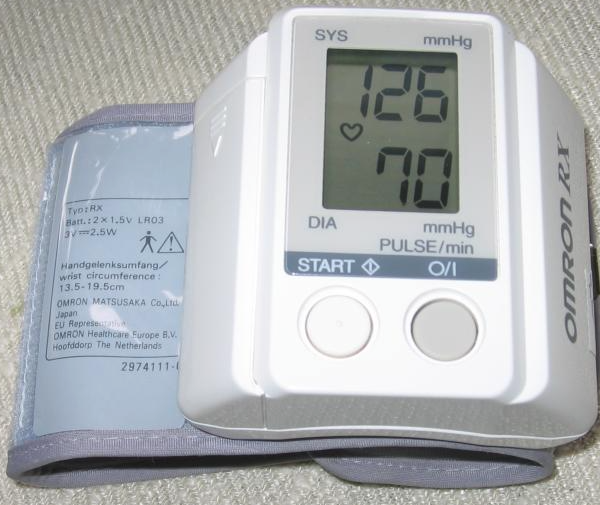
\includegraphics[scale=0.3]{PressureSensors/ton}}
\caption{Sphygmomanometer\label{fig:ton} \cite{ton}}
\end{figure}

\subsection{Industry and factories}

Pressure sensors is very important part of industrial control systems. The sensors allow to maintain large chemical reactions in suitable for process condition, reduce risk of explosions for pressure vessel, monitor storage system for liquids and gases (available volume and partial pressures). In addition this kind of sensor are very important for diagnostics of tubes and filtering systems.

\subsection{Marine and aviation} 

Plane's contraction has several application for pressure sensors, first of all they are used to provide nominal ground like breathing conditions inside, they are also in construction of altimeters especially old-fashion ones. \cite{alt} The atmospheric altimeters are able to measure an altitude via difference between reference air pressure at 0 MAMSL and current value. A typical display of analogue altimeter is shown on picture \ref{fig:alt}.\\

Submarines use sensor in very same way with planes, they use pressure to measure depth, they also use pressure sensors to evaluate amount of compressed air in tanks and maintain right condition inside living areas. \cite{app}

\begin{figure}[H]
\centerline{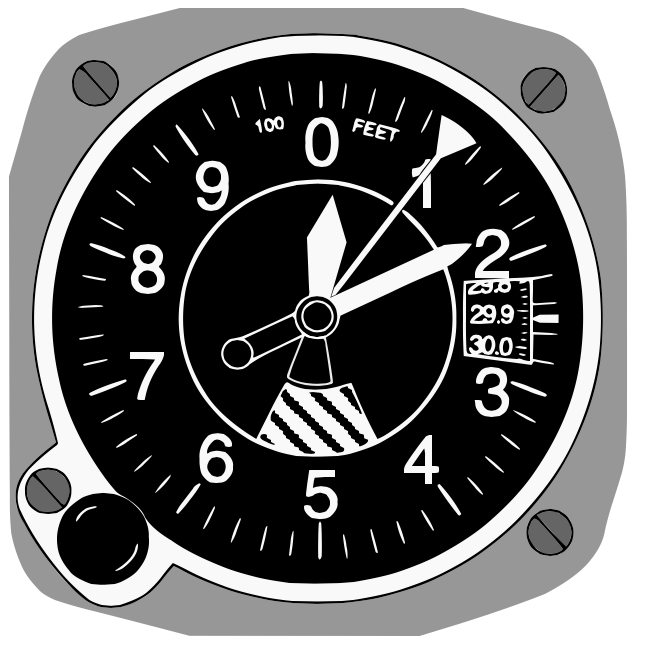
\includegraphics[scale=0.3]{PressureSensors/alt}}
\caption{Screen of analogue altimeter \label{fig:alt} \cite{alt}}
\end{figure}

\subsection{The weather forecasting}

An air flow is always going for high to low pressure area, it makes pressure sensors one of the main tool for the weather forecasting. A network of barometers distributed around wide area allows accurately predict wind and cyclone's velocity.

\subsection{Research}

As any other sensor pressure ones have wide area of original application for different types of research outside of their traditional range of usage, mention above.

\subsection{Robotics}

Robots need to have hand to be able to manipulate things around them. Pressure sensor is very important part of the hand, because it allows to make more precise control over grip. Pressure monitoring can prevent damage to goods and predict false. Robots usually use specially constructed pressure sensors called tactile sensors. Actually tactile sensor is set of pressure sensors, the type of devises gained a lot from MEMS approach, because it allows to stick tougher much bigger number of pressure sensors and in result have better resolution. The tactile sensors can also include temperature and other types of sensors to get information about the surface.\cite{app}

\begin{figure}[H]
\centerline{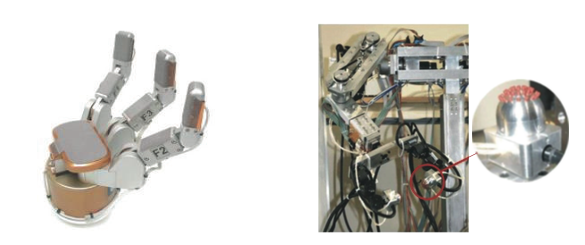
\includegraphics[scale=0.7]{PressureSensors/app}}
\caption{Robo-hands examples\label{fig:app} \cite{app}}
\end{figure}

\section{Markets and history of the pressure sensor}

\subsection{Early development}

The development of pressure sensors was started from in early 50-s from piezoresistive semiconductors. The research proofed that piezoresistive materials are able to change resistance linearly to the amount of applied stress. The main advantage of the technology was low price and small size of the devise.\\

\subsection{80-s}

The technology was improved in 1985, by founding of silicon on insulator (SOI) material. This kind of sensors was even small, it also required much more simple electronics to handle measurements and as result the sensors were cheaper.\\

\subsection{90-s}

Mono mode optical Fabry-Perot interferometer was developed, the invention was key to design of a new resonant differential pressure sensor. The sensor is based on mix of optical and ultrasound effects, that's why very stable and accurate.\\

Piezoresistive sensor was also significantly improved by high pressure protection, this type of sensors started to be suitable for a wide range of very high pressures. Capacitor pressure sensors started to be produced, they have had better performance for low temperature environment, than piezoresistive ones.

\subsection{00-s}

At early 00-s, new CCD sensors and Wollaston prism helped to develop self-calibrated optical pressure sensor. A Fabry-Perot cavity pressure sensor was improved by micromachining techniques at 2003. \\

At 2006 brand-new Fabry-Perot interferometer optical fibre pressure sensor was released. The sensor is based on phase demodulation method. The data processing of for the technique includes Fourier transformation of the Phase demodulation method, which allows to eliminate the light source intensity variation errors.\\

Mesa diaphragm type optical MEMS pressure sensor was presented in 2009, the general concept is based on Fabry-Perot interference. In 2009, Extrinsic Fabry-Perot Interferometric (EFPI) pressure sensor was improved by high temperature immunity.\cite{hist}

\section{Fabrication of the pressure sensor}

 Different types of pressure sensors have very different fabrication process and I am not able to explain all of them in high in details, but I will try to highlight the most typical things for the mechanism. As many other types if MEMS devises pressure sensors are usually based on semi-conductive technologies. The general structure of the sensor is usually created with help of SU-8 Lithography Process, the technology is very helpful in building of tiny structures.\\
 
 Let's take a little bit deeper look into construction of piezoresistive sensors. The production starts from creation of a cavity by surface micro-machining process. After that the cavity is covered by diaphragm made from polysilicon layer or a low stress nitride. The piezoresistive material is placed on top of the diaphragm. The sensor fabrication process is shown on Pic. \ref{fig:fabrik}.\cite{fabrik}\\
 
 \begin{figure}[H]
\centerline{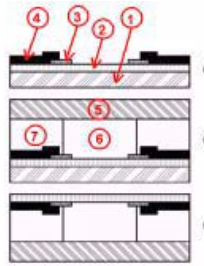
\includegraphics[scale=0.5]{PressureSensors/fabrik}}
\caption{Fabrication process of the pressure sensor: 1) silicon wafer, 2) polysilicon diaphragm, 3) piezoresistive sensor, 4) metal lead, 5) Pyrex glass, 6) cavity and 7) SU-8 layer\label{fig:fabrik}}
\end{figure}

\section{Commercial manufacturers of the pressure sensor}

There are many manufactures of pressure sensors, but I will be focused on three key player of the market.

\subsection{Honeywell}

Multinational conglomerate from UAS, was found at 1906, Wabash, Indiana by Mark C. Honeywell. The company has approximately 130,000 whole over the world and almost half of them are located in States. The main office is located in  Morristown, New Jersey. The CEO is David M. Cote.\\

The company was initially focus on thermostats and control systems for electric motors, but the area was extended to computing by joint venture with Raytheon.\\

Honeywell produce a lot of goods for army, aircraft and NASA. \cite{honey}

 \begin{figure}[H]
\centerline{
\includegraphics[scale=0.5]{PressureSensors/honey}}
\caption{The logo of Honeywell\label{fig:honey}}
\end{figure}

\subsection{Omron}

The company was found in Osaka, at 1933 as Tateisi Electric Manufacturing Co. Omoron was always focused on support of an industry with innovative solutions and advanced technologies. Talent and philosophy of the founder, Kazuma Tateisi, have had very strong influence to the corporative culture of OMRON.\cite{omron}\\

\begin{figure}[H]
\centerline{
\includegraphics[scale=1]{PressureSensors/omron}}
\caption{The logo of Omron\label{fig:omron}}
\end{figure}

The Omron history in milestones:


\begin{itemize}
\item 1933 - started production of X-ray timers,
\item 1959 - "OMRON" trademark established.
\item 1960 - started production of world first non-contact switch 
\item 1960 - developed the world's first automated traffic signal 
\item 1969 - released the smallest in the world electronic calculator
\item 1971 - the world first online automated cash dispenser created
\item 1987 - developed the world's first ultra-high-speed fuzzy logic controller 
\item 1991 - In-line inspection system released
\item 1998 - Created machine for identification of capable counterfeit notes in various currencies
\item 2007 - The world's first real-color 3D Vision Sensor is created
\end{itemize}

\subsection{STMicroelectronics}

STMicroelectronics is one of the largest producer of semiconductors in the world. In 2014 year, it had net revenues of US\$ 7.40 billion. The company provides wide range of products.\\

STMicroelectronics has various solutions for automotive products, embedded-processing solutions, sense and power technologies. They are also a big supplier of MEMS and advance analogues solutions. The Embedded Processing Solutions contains digital consumer, microcontrollers and image signal processors.\\

Products of the company is used in almost every microelectronic device which brings positive contribution to people's lives. They are leaders at several markets:
\begin{itemize}
\item Semiconductors for industrial applications
\item Inkjet print-heads
\item MEMS (Micro-Electro-Mechanical Systems)
\item Automotive integrated circuits
\item Computer peripherals
\item Chips for wireless and mobile applications 
\item And much more...
\end{itemize}

In 1987, SGS Microelettronica of Italy and Thomson Semiconducteurs of France were merged into one company named STMicroelectronics. The company has about 43,600 employees, 11 main factories, R\&D centres in 10 counters and sales offices whole around the world.\\

21\% of revenue is spent for R\&D and about 20\% of employees are working at the field. ST is the most innovative companies in the field, it has almost 15 000 patents and pending applications in 9 000 of patents family. They have made 500 applications for brand-new patents for 2014.\cite{st}\\

The STMicroelectronics logo is shown on Pic. \ref{fig:st}.

\begin{figure}[H]
\centerline{
\includegraphics[scale=0.5]{PressureSensors/st}}
\caption{The logo of STMicroelectronics\label{fig:st}}
\end{figure}


\section{Presentation of a commercial pressure sensor with main specifications}

I want to introduce you MEMS Gauge Pressure Sensor Featuring Small Size and Low Power Consumption, pic. \ref{fig:sensor}. Typical the sensor is used for medical equipment, home appliance, air movement control, level indicators, leak detection or pressure control.\\

The sensor is gauge piezopesistive and can be used for non-corrosive, dust free gases.\\ 

\begin{figure}
\centerline{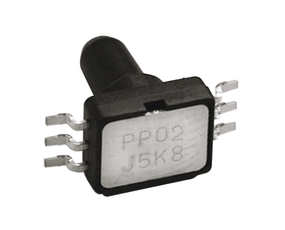
\includegraphics[scale=1]{PressureSensors/sensor}}
\caption{MEMS Gauge Pressure Sensor Featuring Small Size and Low Power Consumption\label{fig:sensor}}
\end{figure}

The main features:
\begin{itemize}
\item Size - 6.1 × 4.7 × 8.2 mm (L × W × H).
\item Piezo Resistive element provides electrical characteristics that are superior to capacitive type pressure sensors.
\item The range of measurable pressure vary for different specifications: 
\begin{itemize}
\item  0 to 37 kPa for 2SMPP-02
\item -50 to 50 kPa for 2SMPP-03
\end{itemize}
\item Low Power consumption -  0.2 mW
\item Low Temperature Influence
\item RoHS Compliant
\item SOP stricture
\item Price 6.25\euro
\end{itemize}

The sensor has to be connected according with schema on pic. \ref{fig:terminal}. The pressure can be calculated in according with output voltage, look at transfer function on Pic. \ref{fig:grapth}.\cite{ds}

\begin{figure}
\centerline{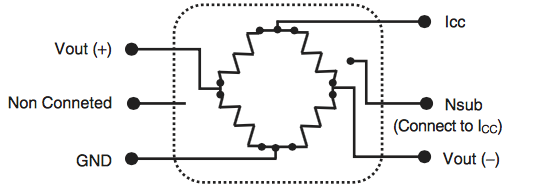
\includegraphics[scale=0.5]{PressureSensors/terminal}}
\caption{Conection of the sensor\label{fig:terminal}}
\end{figure}
\begin{figure}
\centerline{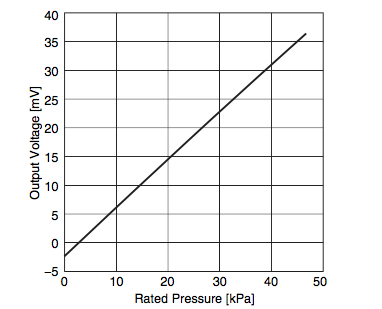
\includegraphics[scale=0.5]{PressureSensors/grapth}}
\caption{Sensor's transfer function\label{fig:grapth}}
\end{figure}

\subsection{Testing environment}

In according with definition the best way to test the sensor is to apply some known amount of force to some well known area. I would prefer to you some cargo as force source, because it would be very easy to calculate the pressure in according with the weight of object with well known mass. 

\section{Conclusion}

We are surrounded my pressure sensors. The type of devises has long history, but it become especially popular in its the MEMS realisation. This type of sensors is used in wide range of applications. Many different solutions are available in the market, the devices can have different construction and physical principle behind, because there is no best solution, every approach has its own advantage and suits well for specific case.\\

Pressure sensors are mainly used at:

\begin{itemize}
\item touch detection
\item auto-mobile industry
\item research
\item factories
\item marina and aviation
\item forecasting
\item robotics
\item medicine
\end{itemize}

Main suppliers of MEMS pressure sensors are huge international companies specialised on microelectronics and sensors, because production of the devises is based on semi-conductive technologies and lithography. \\

It is externally difficult to over estimate importance of pressure sensors and imagine modern technologies without them.

\newpage

% BIBLIOGRAPHY ****************************************************************************************************************

\newpage

\begin{thebibliography}{1}

   \bibitem{spd} Factsheet SPD family information "Introduction to the principals of Smart Pressure Devices", March 9, 2011
  
   \bibitem {types}  Journal of Sensors "Pressure Sensor: State of the Art, Design, and Application for Robotic Hand"
   
   \bibitem {piez}  Steve Carter, Alex Ned, John Chivers, Andy Bemis "Selecting Piezoresistive vs. Piezoelectric Pressure Transducers"
   
   \bibitem {optics} Yuerui Lu, and Amit Lal, SonicMEMS Laboratory, School of Electrical and Computer Engineering, Cornell University, Ithaca, NY, "PHOTONIC CRYSTAL BASED ALL-OPTICAL PRESSURE SENSOR" 
   
  \bibitem {ultrasonic}  Takayuki Tanaka, Shigeki Hori, Ryusuke Yamaguchi, University of Electro-Communications "Ultrasonic Sensor Disk for Detecting Muscular Force".
  
  \bibitem {app} Article : "Pressure Sensors"  -  engineersgarage.com (08.11.2015)
  
  \bibitem {inf} Infineon Technologies AG "New Applications for Integrated Pressure Sensors" 
  
  \bibitem {apple} Apple 3D Touch Technology - apple.com/iphone-6s/3d-touch
  
  \bibitem {touch} Robin Granger, MEng, Roke Manor Research Chemring Technology Solutions Romsey, UK"Modelling RF Losses in Touchscreens"
  
  \bibitem {wacom} Wacom graphical tablets website wacom.com
  
  \bibitem {alt} en.wikipedia.org/wiki/Altimeter
  
  \bibitem {ton} en.wikipedia.org/wiki/Sphygmomanometer
  
  \bibitem {hist} International Journal of Emerging Technology and Advanced Engineering "Survey on Pressure Sensors in the Previous Decades"
  
  \bibitem {fabrik} C. W. Liu1, H. S. Ko2, Chie Gau2, C. G. Liu3, National Nano Device Laboratory "Micro Pressure Sensor Fabrication without Problem of Stiction for a Wider Range of Measurement"
  
  \bibitem {honey} Wikipedia about Honeywell - en.wikipedia.org/wiki/Honeywell
  
  \bibitem {omron} Official website - omron.com
  
  \bibitem {st} STMicroelectronics official website - st.com
  
  \bibitem {ds} MEMS Gauge Pressure Sensor 2SMPP datasheet
  
  \bibitem {mems} 1999 International Symposium on Advanced Packaging Materials "Challengesinthe Packaging of MEMS"

  \end{thebibliography}

\end{document}
